\documentclass[11pt,a4paper]{article}
\usepackage[T1]{fontenc}
\usepackage[utf8]{inputenc}
\usepackage[margin=1in]{geometry}
\usepackage{amsmath,amssymb,amsthm}
\usepackage{mathpartir}
\usepackage{stmaryrd}
\usepackage{booktabs}
\usepackage{tabularx}
\usepackage{array}
\usepackage{longtable}
\usepackage{enumitem}
\usepackage{listings}
\usepackage{xcolor}
\usepackage[expansion=false]{microtype}
\usepackage{tikz}
\usetikzlibrary{arrows.meta,positioning,fit,calc}
\usepackage[htt]{hyphenat}
\usepackage[hidelinks,pdftitle={F1R3COMB: a compiler from kernel rho to the name-free rho combinators}]{hyperref}
\setlength{\emergencystretch}{3em}

\newcommand{\code}[1]{\texttt{#1}}
\newcommand{\Comb}{\textsc{F1R3Comb}}
\newcommand{\Kind}{\textsc{K1ndl1ng}}
\newcommand{\Camp}{\textsc{CampF1R3}}
\newcommand{\Bell}{\textsc{B3ll0ws}}
\newcommand{\Fx}{\textsc{F1R3x}}
\newcommand{\Rhobots}{\textsc{Rhobots}}
\newcommand{\MUST}{\textsc{must}}
\newcommand{\MUSTNOT}{\textsc{must not}}
\newcommand{\SHOULD}{\textsc{should}}
\newcommand{\SHOULDNOT}{\textsc{should not}}
\newcommand{\MAY}{\textsc{may}}

\newcommand{\quo}[1]{@#1}
\newcommand{\drp}[1]{{*}#1}
\newcommand{\inp}[3]{\mathsf{for}(\,#1 \leftarrow #2\,)#3}
\newcommand{\out}[2]{#1!(#2)}
\newcommand{\nil}{\mathbf{0}}
\newcommand{\enc}[1]{\llbracket #1 \rrbracket}
\newcommand{\nequiv}{\equiv_{\mathcal{N}}}
\newcommand{\bisim}{\approx}
\newcommand{\nms}[1]{\mathcal{N}^{*}(#1)}
\newcommand{\Nsort}{\mathsf{N}}
\newcommand{\Psort}{\mathsf{P}}

\newcommand{\mm}{\mathsf{m}}
\newcommand{\dd}{\mathsf{d}}
\newcommand{\kk}{\mathsf{k}}
\newcommand{\fw}{\mathsf{fw}}
\newcommand{\bl}{\mathsf{b}_{\mathsf{l}}}
\newcommand{\br}{\mathsf{b}_{\mathsf{r}}}
\newcommand{\sy}{\mathsf{s}}
\newcommand{\ev}{\mathsf{e}}
\newcommand{\qq}{\mathsf{q}}
\newcommand{\cons}{\mathsf{cons}}
\newcommand{\red}{\longrightarrow}
\newcommand{\wred}{\longrightarrow^{*}}
\newcommand{\scong}{\equiv}
\newcommand{\Atm}{\mathcal{A}}
\newcommand{\comps}[1]{\lvert #1 \rvert}
\newcommand{\rcp}[1]{\langle\!\langle #1 \rangle\!\rangle}
\newcommand{\Cl}{\mathrm{Cl}}

\theoremstyle{definition}
\newtheorem{definition}{Definition}[section]
\newtheorem{requirement}[definition]{Requirement}
\newtheorem{decision}[definition]{Decision}
\newtheorem{obligation}[definition]{Obligation}
\newtheorem{hazard}[definition]{Hazard}
\newtheorem{erratum}[definition]{Erratum}
\newtheorem{remark}[definition]{Remark}
\newtheorem{example}[definition]{Example}
\theoremstyle{plain}
\newtheorem{proposition}[definition]{Proposition}
\newtheorem{lemma}[definition]{Lemma}

\lstset{
  basicstyle=\ttfamily\footnotesize,
  columns=fullflexible,
  keepspaces=true,
  breaklines=true,
  frame=leftline,
  framesep=6pt,
  xleftmargin=8pt,
  rulecolor=\color{black!30},
  showstringspaces=false,
}

\title{\textbf{\Comb}\\[1mm]
\large A compiler from kernel rho to the name-free rho combinators,\\
and a machine that runs the result\\[2mm]
\normalsize Specification v0.2}
\author{F1R3FLY.io}
\date{22 September 2026}

\begin{document}
\maketitle

\begin{abstract}
\noindent
\emph{Name-free combinators for the rho calculus} (draft~3, \cite{draft3})
repairs the combinator calculus of \cite{rhocomb}, supplies the
rho-to-combinator translation the original promised and never gave, and proves
it correct as full abstraction relative to encoded contexts. Its companion
\cite{logic} gives the spatial-behavioural logic over the same calculus.
Nothing executes either. The \code{campf1r3} workspace supplies, for kernel
rho, everything a compiler of this shape needs on the source side --- a parser
and a normaliser for K0 \cite{k1ndl1ng}, a store \cite{campf1r3}, an
interpreter \cite{bytecode} --- and nothing on the target side. This document
specifies the arrow between them: five crates that take a K0 term to a
combinator term, and run it.

Draft~3 now presents the target as an operational theory over two sorts and
offers two sound presentations, A and B, differing in whether
$\drp{\quo{p}} = p$ is an equation and hence in whether a message payload is
a name or a process. A compiler cannot hold both: the term type, the store's
datum type, the tag table and the decision procedure for $\nequiv$ all differ.
Section~\ref{sec:which} takes presentation~A, for five reasons of which three
are decisive --- the logic is a logic for A and cannot tell a store from a
message under B \cite[Rem.~2.5]{logic}; quotation is injective only under A
\cite[Prop.~2.10]{logic}, and \Camp{} keys channels by the encoding; and the
translation of \cite[Def.~6.6]{draft3} is written in A's notation. It also
records that the implementation argument of \cite[\S4]{draft3}, which reads
the F1R3FLY normaliser as evidence for B, does not survive contact with the
code, and points the other way.

Two findings from v0.1 survive unchanged and are restated:
\cite[Def.~6.1]{draft3}'s seed powers are constructible at run time by
$\cons_{\mm}$, so freshness fails against the calculus's own constructors
(Erratum~\ref{err:seed}); and \Camp{} keys channels by the encoding, so the
compiler must be canonical, not merely correct up to bisimilarity, which
Decision~\ref{dec:seed} secures. One decision from v0.1 is reversed:
$\qq$ \emph{must} carry a process, not a name, because the sort asymmetry
between $\mm$ and $\qq$ is the whole of what makes storage visible to the
logic. Section~\ref{sec:v1delta} lists the changes.
Key words \MUST, \MUSTNOT, \SHOULD, \MAY{} are used in the sense of RFC~2119.
\end{abstract}

\tableofcontents

%======================================================================
\section{Purpose and scope}\label{sec:purpose}

\subsection{The gap}

Draft~3 ends with a translation $\enc{-}_{s}$ from the rho calculus into the
repaired combinators, a release lemma that fixes the reduction sequence
following a communication, and a full abstraction theorem relative to encoded
contexts. The translation is defined on paper, by a table of five occurrence
kinds and four clauses. It has never been run, and the properties that a
paper translation is allowed to leave up to bisimilarity --- which seed, which
order of emission, which representative of a constructed name, and now which
presentation --- are properties an implementation is not allowed to leave
open, because they decide whether two independently compiled terms can speak
to one another.

On the other side, the \code{campf1r3} workspace (the repository
\code{F1R3FLY-io/campf1r3}, crate family \code{f1r3-executive}) is a complete
executive for kernel rho: \code{k1ndl1ng-parse} and \code{k1ndl1ng-norm} take
text to a canonical normal form, \code{campf1r3-core} is the store,
\code{b3ll0ws} interprets the normal form directly, and \code{f1r3x} drives
them. It knows nothing of combinators.

\Comb{} is the missing arrow, plus the smallest machine that can run its
output.

\subsection{What exists today}

\begin{center}
\begin{tabularx}{\linewidth}{@{}l>{\raggedright\arraybackslash}X@{}}
\toprule
Artefact & What it gives this project\\
\midrule
\code{publications/rho-combinators/rho-combinators-draft3} & The target
calculus as an operational theory (\S3.2--3.3, Def.~3.1, Def.~3.3), the two
presentations (\S3.3) and the argument between them (\S4), the translation
(Def.~6.6, Table~1), the correctness lemmas (\S7), the expressiveness lattice
(\S9), the constructors-only presentation (\S10)\\
\code{publications/rho-combinators/rhocomb-logic} (draft~2) & The logic over
the combinators; the presentation decision (Dec.~2.3), what B costs the logic
(Prop.~2.4, Rem.~2.5), drop elimination (Lem.~2.8), $\nequiv$ decided
(Prop.~2.10), occupancy in linear time (Thm.~6.5)\\
\code{publications/campf1r3/k1ndl1ng-spec} & K0 = pure rho; the AST, the
normal form, its encoding, its hashing, the congruence requirement
(Def.~2.6, Req.~2.7, Prop.~6.9)\\
\code{publications/campf1r3/campf1r3-spec} & The store: $D$, $W$, $I$,
produce/consume/install as single cuts, joins, profiles, replay\\
\code{publications/campf1r3/bytecode-or-normal-form} & Why code must never be
a channel key unless the compiler is canonical (\S\,identity); the backend
seam\\
\code{campf1r3} (the repository) & \code{k1ndl1ng-ast}, \code{k1ndl1ng-parse},
\code{k1ndl1ng-norm}, \code{campf1r3-core}, \code{k1ndl1ng-campf1r3},
\code{b3ll0ws}, \code{f1r3x}, \code{f1r3x-ffi}, \code{f1r3x-wasm}; no external
dependencies at all\\
\bottomrule
\end{tabularx}
\end{center}

\subsection{Nomenclature}\label{sec:nomen}

\begin{center}
\begin{tabularx}{\linewidth}{@{}l>{\raggedright\arraybackslash}X@{}}
\toprule
Term & Meaning in this document\\
\midrule
\emph{source} & K0 of \cite{k1ndl1ng}: $\nil$, par, monadic send, monadic
receive on a name variable, unquote, quote. The rho calculus of
\cite[\S2]{draft3}, modulo Obligation~\ref{obl:srcagree}\\
\emph{target}, \emph{the combinators} & The theory of \cite[\S3]{draft3}:
two sorts, thirteen atom shapes, $\nil$, par, quote and drop, no binders, no
name hiding\\
\emph{presentation A}, \emph{B} & The two variants of \cite[\S3.3]{draft3};
A adds $\drp{\quo{p}} = p$ and sorts message payloads as names, B omits it
and sorts them as processes\\
\emph{atom} & One combinator occurrence. $\ev$ is an atom; $\drp{-}$ is a
process former and is \emph{not} $\ev$ (\cite[\S3.2]{draft3})\\
\emph{message} & $\mm(a,v)$; the only loud value-bearing atom\\
\emph{store} & $\qq(a,p)$, readable only by a forwarder\\
\emph{router} & $\dd,\kk,\fw,\bl,\br,\sy$\\
\emph{constructor} & $\cons,\cons_{\mm},\cons_{\dd},\cons_{\sy}$, and under
the \code{shortcuts} feature $\cons_{\ev},\cons_{\fw}$\\
\emph{seed} & A name $s$ fresh for the term being translated; $s^{w}$ its
powers, indexed by a binary string\\
\emph{proxy} & A constructed name $c_{i}$ standing at one occurrence of a
bound name in a released continuation\\
\emph{link} & The atom emitted for one occurrence, per Table~\ref{tab:links}\\
\emph{deploy} & Installing a compiled term into the machine's store\\
\bottomrule
\end{tabularx}
\end{center}

\noindent
The product name is \Comb, written \code{f1r3comb} in crate names and
\code{comb} in \Fx{} subcommands. The calculus is \emph{the rho combinators},
never \emph{rhocomb}, which names the earlier draft \cite{rhocomb}.

\subsection{Goals}

\begin{enumerate}[leftmargin=1.6em]
\item A total, canonical, provably terminating compiler from K0 normal forms
to combinator terms, implementing \cite[Def.~6.6]{draft3} with every degree of
freedom in that definition closed --- including the choice of presentation.
\item A target representation with its own canonical encoding and content
hash, in the same style and the same tag-space discipline as \Kind's, so that
$\nequiv$ on target names is a 32-byte comparison.
\item A machine that runs target terms by instantiating \Camp{} --- no
spatial matcher, no substitution, no de Bruijn --- with the same determinism
and replay guarantees \code{campf1r3} already offers.
\item Differential testing against \Bell: the same source program, run both
ways, agreeing on the observations an encoded context can make.
\item A term type and an occupancy report that \cite{logic} can build on
without a compiler.
\item The same portability envelope as the rest of the workspace: no external
dependencies, \code{forbid(unsafe\_code)}, WebAssembly-clean.
\end{enumerate}

\subsection{Non-goals}\label{sec:nongoals}

\begin{enumerate}[leftmargin=1.6em]
\item \textbf{The logic itself.} \cite{logic} specifies satisfaction,
characteristic formulae, occupancy and a model checker. \Comb{} \MUSTNOT{}
implement any of them. It \MUST{} expose the atom multiset and the lattice
point (Section~\ref{sec:lattice}), which is what the occupancy checker needs
from a compiler, and nothing more.
\item \textbf{K1 and K2.} Polyadic send and receive, joins, persistence, peek,
\code{new}, name patterns and guards are outside the source language. The
compiler \MUST{} reject them with the level diagnostic of
\cite[Req.~2.1]{k1ndl1ng} rather than attempt a translation.
\item \textbf{The $\pi$ route.} Composition with \cite{nowns} is a later
question.
\item \textbf{Decompilation.} No combinator-to-rho direction is specified.
\item \textbf{Cost accounting.} Out of scope; Section~\ref{sec:runtime}
leaves the \Camp{} observer seam open so it can be added later.
\item \textbf{Optimisation beyond \cite[Rem.~6.7]{draft3}.} The three
shortcuts named there are the whole of the optimisation budget for v1.
\end{enumerate}

%======================================================================
\section{Which presentation}\label{sec:which}

\subsection{The choice cannot be deferred}

\cite[\S3.3]{draft3} gives two presentations, both sound, and
\cite[Rem.~3.2]{draft3} shows they cannot be mixed piecemeal. For a paper this
is a pleasant degree of freedom: \cite[Def.~3.3]{draft3} records that no rule,
lemma or proof in the note distinguishes them. For a compiler it is not a
degree of freedom at all. Every artefact this specification names differs
between them:

\begin{center}
\begin{tabularx}{\linewidth}{@{}l>{\raggedright\arraybackslash}X>{\raggedright\arraybackslash}X@{}}
\toprule
& Presentation A & Presentation B\\
\midrule
$\mm$ payload sort & $\Nsort$ & $\Psort$\\
$\qq$ payload sort & $\Psort$ & $\Psort$\\
$\mathsf{eval}$ & $\ev(a) \mid \mm(a,v) \red \drp{v}$ &
  $\ev(a) \mid \mm(a,p) \red p$\\
$\drp{-}$ in a target term & eliminable; absent from every normal form
  (\cite[Lem.~2.8]{logic}) & irreducible; needed, since $\mm(v,\drp{x})$ is how
  a name is sent\\
$\quo{-}$ injective & yes, on normal forms (\cite[Prop.~2.10]{logic}) &
  no (\cite[Prop.~2.4(ii)]{logic})\\
$\nequiv$ decided by & byte equality of the canonical encoding &
  $\quo{\drp{a}} \to a$ normalisation, then comparison; strictly coarser than
  A's equality\\
Store datum type & \code{Loud(CName)} $\mid$ \code{Quiet(Term)} &
  \code{Loud(Term)} $\mid$ \code{Quiet(Term)}\\
Canonical form & flat multiset of atoms & multiset plus a descent production
  for $\drp{\nu}$\\
Logic support & full & needs a receptivity primitive before it can say
  anything about storage (\cite[Rem.~2.5]{logic})\\
\bottomrule
\end{tabularx}
\end{center}

\begin{decision}[\Comb{} implements presentation A]\label{dec:presA}
The compiler, the term type, the encoding and the machine implement
presentation~A. B is a seam, not a default (Requirement~\ref{req:pseam}).
\end{decision}

\subsection{Why A}

\begin{enumerate}[leftmargin=1.8em]

\item \textbf{The logic needs it, and the logic is the other consumer of this
term type.} \cite[Dec.~2.3]{logic} states satisfaction against A and says the
choice is forced rather than convenient: the grammar's $\mm(\nu_1,\nu_2)$
against $\qq(\nu,\phi)$ asymmetry exists only under A. Under B the two
productions coincide, and by \cite[Rem.~2.5]{logic} the logic cannot
distinguish a store from a message \emph{at all} --- what separates them is a
receptivity statement, which is not derivable from the context modality and
negation, and is open item~5 of that note. Requirement~\ref{req:indep} makes
\code{f1r3comb-term} usable by the logic tooling without the compiler; a term
type built for B would hand that tooling a problem it does not currently know
how to solve.

\item \textbf{Channel identity requires injective quotation.} \Camp{} keys a
channel by the content hash of its encoding, and \cite[Req.~2.7]{k1ndl1ng}
requires equality of terms, of encodings and of hashes to agree. Under A,
drop elimination (\cite[Lem.~2.8]{logic}) is terminating and confluent, normal
forms are drop-free, and $\quo{-}$ is injective on them
(\cite[Prop.~2.10]{logic}): equality of names is equality of bytes, full stop.
Under B, $\drp{\quo{p}}$ and $p$ are distinct processes with equal quotations,
so two distinct payloads live at one key, and the agreement
\cite[Req.~2.7]{k1ndl1ng} asks for holds in one direction only. It is
recoverable --- normalise $\quo{\drp{a}} \to a$ and compare --- but it is a
second decision procedure where A has none.

\item \textbf{The translation is written in A.} \cite[Def.~3.3]{draft3} says
payloads are written in A's notation, $\mm(a,\quo{p})$, and \S6 uses that
notation throughout: $\enc{\out{x}{P}}_{s} = \mm(\enc{x},\quo{\enc{P}_{s^0}})$,
the gate $\qq(b,S)$ with a process payload, the constructor rules with
$\mm(a,\quo{p})$ premises. Implementing A is transcription; implementing B is
re-derivation of every clause, with the sort of each payload checked by hand.

\item \textbf{The representation is smaller.} No drop node in the term type,
no descent production in any traversal, canonical forms that are flat
multisets of atoms (\cite[Prop.~2.4(iii)]{logic} is the statement of what B
costs here).

\item \textbf{The existing normaliser already implements A on the source
side.} \code{k1ndl1ng\_norm::Norm::eval} applies $\drp{\quo{P}} \to P$ at
construction, and \cite[Def.~2.6]{k1ndl1ng} states the source congruence with
that clause in it. Choosing A makes one equation govern both sides of the
compiler.

\end{enumerate}

\subsection{The implementation argument in \cite[\S4]{draft3}}
\label{sec:s4rebuttal}

\cite[\S4]{draft3} argues for B from the implementation: the F1R3FLY
implementation normalises on decode, what is handed back has been rearranged
and bound variables replaced by de Bruijn indices, neither transformation is
derivable from the equations, so under A the implementation is unsound for its
own theory and under B it is sound. The conclusion drawn is that the
implementation is evidence for B.

That argument does not hold against the code, on three counts, and this
specification records them because \S4 is the paper's principal argument for B
and Decision~\ref{dec:presA} goes the other way.

\begin{enumerate}[leftmargin=1.8em]
\item \textbf{The rearrangement is the monoid laws.} What
\code{k1ndl1ng-norm} does to a parallel composition is sort its components by
bytewise comparison of their encodings. Sorting a multiset is exactly
commutativity and associativity of $\mid$, which \cite[Def.~3.1]{draft3} gives
as \emph{common} to both presentations. So this transformation is derivable
from the equations, and the decoded process is equal to the quoted one, not
merely bisimilar to it.

\item \textbf{De Bruijn indices are a source-calculus feature.} The
combinators have no binders --- \cite[Def.~3.1]{draft3} says so, and it is the
point of the whole exercise. \code{k1ndl1ng-norm} assigns de Bruijn indices to
the binders of a kernel rholang \code{Receive}. A decoded \emph{combinator}
term has no bound variable to index, so the transformation never applies to
the thing \S4 is talking about.

\item \textbf{The one presentation-specific step the code performs is A's
equation.} \code{Norm::eval} rewrites $\drp{\quo{P}}$ to $P$. That is
$\drp{\quo{p}} = p$, which A asserts and B denies. Under A it is a sound
normalisation; under B it identifies two processes the theory keeps apart, and
is the one place the implementation would be unsound.
\end{enumerate}

\noindent
Taken together, the evidence \S4 appeals to points at A. \S4's structural
argument --- that decoding is an event under B and an identity under A, and
that only B lets a decoder return a bisimilar representative --- stands
untouched; it is an argument about what a future implementation \emph{may}
do, not about what this one does.

\begin{remark}[What A gives up, and what it does not]
\label{rem:whatAcosts}
A forfeits the decoder's freedom to return an optimised representative. The
concrete thing that freedom would buy is a backend that discharges the
administrative forwarders of the link expansion (\cite[Lem.~7.4]{draft3}) at
decode time, handing back a smaller bisimilar term. Nothing in \code{campf1r3}
does this today, and \Bell's \code{Direct} backend substitutes into the normal
form and takes its top-level components without optimising. Should such a
backend be wanted, it needs B, and that is the one development to watch. A
does \emph{not} cost anything in cost accounting: $\mathsf{eval}$ is a
reduction step under both presentations and is equally chargeable; what A
fixes is only the identity of the result, not whether producing it is an
event.
\end{remark}

\subsection{The seam}

\begin{requirement}[Presentation is a compile-time parameter]\label{req:pseam}
The presentation \MUST{} be a cargo feature, \code{presentation-b}, off by
default, and the crates \MUST{} be structured so that turning it on changes
the payload sort of $\mm$, the $\mathsf{eval}$ rule, the presence of the drop
node and the $\nequiv$ decision procedure, and nothing else. It \MUST{} be
recorded in the header of every compiled artefact, and a deploy \MUST{}
diagnose a mismatch (\code{comb-presentation-mismatch}) rather than proceed:
under B the same source compiles to a term with different bytes and a
different hash, so two deploys that disagree about the presentation cannot
meet, and must be told so.
\end{requirement}

\begin{requirement}[No piecemeal mixing]\label{req:nomix}
\cite[Rem.~3.2]{draft3} shows that omitting $\drp{\quo{p}} = p$ while keeping
name-sorted payloads leaves $\mathsf{eval}$ either stuck or ambiguous. The
build \MUST{} therefore couple the equation, the payload sort and the
$\mathsf{eval}$ rule in one feature, and \MUSTNOT{} expose them as three. A
test \MUST{} assert that the feature matrix has exactly two reachable
configurations.
\end{requirement}

%======================================================================
\section{The source language}\label{sec:source}

\subsection{K0 is the paper's rho}

\begin{center}
\begin{tabular}{@{}lll@{}}
\toprule
\cite[Def.~2.1]{draft3} & K0 concrete syntax & \code{k1ndl1ng-norm} \code{Node}\\
\midrule
$\nil$ & \code{Nil} & \code{Nil}\\
$P \mid Q$ & \code{P | Q} & \code{Par(Vec<Norm>)}, sorted, no \code{Nil}\\
$\out{x}{P}$ & \code{x!(P)} & \code{Send\{chan, persistent:false, args:[P]\}}\\
$\inp{y}{x}{P}$ & \code{for(y <- x)\{P\}} & \code{Receive\{binds:[b], body\}}\\
$\drp{x}$ & \code{*x} & \code{Eval(Name)}\\
$\quo{P}$ & \code{@P} & \code{Name::Quote(Norm)}\\
\bottomrule
\end{tabular}
\end{center}

\begin{requirement}[Source level]\label{req:level}
\Comb{} \MUST{} accept exactly K0, invoking \code{k1ndl1ng\_parse} with
\code{Level::K0}. A \code{Receive} whose bind list has other than one bind, a
bind with other than one pattern, a pattern that is not a name variable, a
\code{Send} with other than one argument, a persistent bang or arrow, a peek,
a \code{New} node, an \code{Unforgeable} name, a \code{Wild}, a
\code{FreeVar} or a \code{FreeName} in a pattern position \MUST{} each produce
a distinct diagnostic (Section~\ref{sec:errors}).
\end{requirement}

\begin{requirement}[Closed input]\label{req:closed}
The term presented to the compiler \MUST{} be closed: no \code{FreeVar}, no
\code{FreeName}. \code{Name::Unforgeable} \MUST{} be rejected at v1, because
the target has no name former for it and inventing one would enlarge the
atom set outside \cite{draft3} and outside $\Atm_{\mathrm{full}}$ as
\cite[Def.~2.1]{logic} counts it. Grounding \MUST{} therefore be by
quotation, and the diagnostic \MUST{} say so.
\end{requirement}

\subsection{Two source presentations, agreeing where it matters}

\cite[\S2]{draft3} states the source congruence \emph{without}
$\drp{\quo{P}} \scong P$ and recovers its work through semantic substitution
(\cite[Def.~2.3]{draft3}). \cite[Def.~2.6]{k1ndl1ng} states it \emph{with}
that clause, and \code{Norm::eval} applies it eagerly. The two source
calculi are therefore not the same calculus, and \Comb{} compiles the second
while claiming the theorems of the first.

\begin{obligation}[The source presentations agree on guarded-drop terms]
\label{obl:srcagree}
For $P$ guarded-drop in the sense of \cite[Def.~2.5]{draft3} --- every
$\drp{x}$ has $x$ bound by an enclosing input --- no subterm $\drp{\quo{Q}}$
occurs in $P$ or in any reduct of $P$ (\cite[Lem.~2.6]{draft3}), so the
rewrite $\drp{\quo{P}} \to P$ never fires and the two congruences coincide on
$P$. This \MUST{} be proved, and it is what licenses compiling a \Kind{}
normal form against \cite[\S2]{draft3}. It is also why nobody has noticed the
mismatch.
\end{obligation}

\begin{requirement}[Guarded-drop check, now a diagnostic]\label{req:guarded}
The compiler \MUST{} verify the guarded-drop property on the \emph{tree},
before normalisation, and \MUST{} report \code{comb-drop-quote} for a literal
$\drp{\quo{Q}}$ and \code{comb-unguarded-drop} for a drop of any other
unbound name. Under Decision~\ref{dec:presA} these are warnings, not errors,
and compilation \MAY{} proceed: the source normaliser and the target theory
both satisfy $\drp{\quo{p}} = p$, so the collapsed term is equal, not merely
bisimilar, to the written one. Under \code{presentation-b} they \MUST{} be
errors, because there the collapse is unsound and
Obligation~\ref{obl:srcagree} is the only thing standing between the compiler
and a source term the theory does not describe.
\end{requirement}

\begin{remark}[v0.1 had this as a hazard]
v0.1 made \code{Norm::eval} the sharpest edge in the specification, on the
grounds that it applies an equation the target must not have. Under
Decision~\ref{dec:presA} the target \emph{does} have that equation, and the
edge is gone: one rewrite, sound on both sides, applied by one function. The
edge returns in full under \code{presentation-b}, which is the substance of
Requirement~\ref{req:nodropB}.
\end{remark}

\subsection{What the normaliser provides}

\begin{center}
\begin{tabularx}{\linewidth}{@{}l>{\raggedright\arraybackslash}X@{}}
\toprule
Property & Use here\\
\midrule
$\enc{P} = \enc{Q} \iff P \scong Q$ (\cite[Prop.~6.9]{k1ndl1ng}) & The input
is a canonical representative of a congruence class, which is what makes
Obligation~\ref{thm:canon} possible\\
Par components sorted by their own encodings & A canonical path index $w$ for
seed allocation (Section~\ref{sec:canon})\\
$\quo{\drp{x}} \to x$, in \code{Norm::quote} & The equation common to both
presentations and to both calculi\\
$\drp{\quo{P}} \to P$, in \code{Norm::eval} & A's equation; see
Obligation~\ref{obl:srcagree}\\
de Bruijn indices for bound names & Occurrence analysis becomes an index
comparison (Section~\ref{sec:occ})\\
BLAKE2b-256 of the encoding & Channel identity, reused verbatim for target
names\\
\bottomrule
\end{tabularx}
\end{center}

\begin{decision}[Compile the normal form, not the tree]
The compiler's input is \code{k1ndl1ng\_norm::Norm}, with the sole exception
of the guarded-drop check of Requirement~\ref{req:guarded}, which needs the
tree. Compiling the tree would make the output depend on the order in which
the author happened to write a parallel composition, and
Obligation~\ref{thm:canon} would be false.
\end{decision}

%======================================================================
\section{The target calculus}\label{sec:target}

\subsection{Formation}

From \cite[\S3.2]{draft3}, with $a,b,c,f : \Nsort$ and $p,q : \Psort$; every
atom has sort $\Psort$ and every argument is a name except the second
argument of $\qq$ and, under B, of $\mm$.

\[
\begin{array}{l@{\qquad}l@{\qquad}l}
 \mm(a,v) & \bl(a,b) & \cons(a,b,c)\\
 \dd(a,b,c) & \br(a,b) & \cons_{\mm}(a,b,c)\\
 \kk(a) & \sy(a,b,c) & \cons_{\dd}(a,b,c,f)\\
 \fw(a,b) & \ev(a) & \cons_{\sy}(a,b,c,f)\\
 \qq(a,p) & \nil \,,\ \ p \mid q & \quo{p} : \Nsort \,,\ \ \drp{a} : \Psort
\end{array}
\]

\begin{requirement}[The drop and the guard are distinct constructors]
\label{req:noconflation}
$\drp{-}$ and $\ev$ \MUST{} be distinct constructors of the target type, and
no code path \MAY{} convert one into the other. This is the whole of the
repair: \cite[Prop.~3.5]{draft3} needs the conflation as a hypothesis, and
with the constructors separate an arbitrary running process cannot match a
guard however many equations the theory carries. The type system enforces it
for free provided $\drp{-}$ is not represented as a nullary-argument $\ev$ or
vice versa; a representation sharing one tag between them \MUSTNOT{} be used
even with a discriminating flag.
\end{requirement}

\begin{requirement}[Rigidity, as a test]\label{req:rigid}
No equation of Definition~\ref{def:teqns} has $\ev$ at its head, and the
rewrite system of Requirement~\ref{req:dropelim} preserves head constructors
other than $\drp{-}$. A test \MUST{} assert the consequence: for every $P$ in
a corpus and every name $a$, the normal form of $P$ is an $\ev$ atom only if
$P$ was written as one. This is Requirement~\ref{req:noconflation} in
executable form.
\end{requirement}

\subsection{Equations}

\begin{definition}[\cite{draft3} Def.~3.1, with A's addition]\label{def:teqns}
$(\Psort,\mid,\nil)$ is an abelian monoid; $\quo{\drp{a}} = a$; and, under
presentation A, $\drp{\quo{p}} = p$.
\end{definition}

\begin{requirement}[Drop elimination]\label{req:dropelim}
Orient the equations left to right: $\drp{\quo{p}} \to p$ and
$\quo{\drp{a}} \to a$. By \cite[Lem.~2.8]{logic} the system is terminating
and confluent and the normal form of a closed term contains no $\drp{-}$. The
smart constructors of \code{f1r3comb-term} \MUST{} apply both rewrites at
construction, exactly as \code{Norm::eval} and \code{Norm::quote} do for the
source, so that every \code{Term} in existence is in normal form and
$\drp{-}$ appears only as a transient argument to a constructor. Every
traversal in the crate \MAY{} therefore assume a flat multiset of atoms.
\end{requirement}

\begin{requirement}[Under B, the opposite]\label{req:nodropB}
With \code{presentation-b} enabled, $\drp{\quo{p}} \to p$ \MUSTNOT{} be
applied, the drop node \MUST{} be retained in the normal form, every traversal
\MUST{} carry a descent case for it (\cite[Prop.~2.4(iii)]{logic}), and the
term type \MUSTNOT{} be routed through \code{k1ndl1ng\_norm::Norm::eval} or
any function that calls it. The \code{presentation-b} build \MUST{} carry a
test asserting that $\drp{\quo{p}}$ and $p$ have different encodings.
\end{requirement}

\subsection{Rules}

\begin{definition}[\cite{draft3} Def.~3.3]\label{def:tred}
Payloads written in A's notation; under B read $\mm(a,p)$ for
$\mm(a,\quo{p})$.
\[
\begin{array}{l}
 \mathsf{dist} : \dd(a,b,c) \mid \mm(a,v) \red \mm(b,v) \mid \mm(c,v)\\
 \mathsf{kill} : \kk(a) \mid \mm(a,v) \red \nil\\
 \mathsf{forward} : \fw(a,b) \mid \mm(a,v) \red \mm(b,v)\\
 \mathsf{bind}_{\mathsf{l}} : \bl(a,b) \mid \mm(a,v) \red \fw(v,b)\\
 \mathsf{bind}_{\mathsf{r}} : \br(a,b) \mid \mm(a,v) \red \fw(b,v)\\
 \mathsf{synch} : \sy(a,b,c) \mid \mm(a,v) \red \fw(b,c)\\
 \mathsf{eval} : \ev(a) \mid \mm(a,v) \red \drp{v}
   \qquad\text{(A)};\qquad \ev(a) \mid \mm(a,p) \red p \quad\text{(B)}\\
 \mathsf{quote} : \fw(a,b) \mid \qq(a,p) \red \mm(b,\quo{p})\\
 \mathsf{make}_{\mid} : \cons(a,b,c) \mid \mm(a,\quo{p}) \mid \mm(b,\quo{r})
   \red \mm(c,\quo{(p \mid r)})\\
 \mathsf{make}_{\mm} : \cons_{\mm}(a,b,c) \mid \mm(a,u) \mid \mm(b,v)
   \red \mm(c,\quo{\mm(u,v)})\\
 \mathsf{make}_{\dd} : \cons_{\dd}(a,b,c,f) \mid \mm(a,u) \mid \mm(b,v)
   \mid \mm(c,w) \red \mm(f,\quo{\dd(u,v,w)})\\
 \mathsf{make}_{\sy} : \cons_{\sy}(a,b,c,f) \mid \mm(a,u) \mid \mm(b,v)
   \mid \mm(c,w) \red \mm(f,\quo{\sy(u,v,w)})
\end{array}
\]
closed under parallel composition and under the equations, with subjects
matched up to $\nequiv$.
\end{definition}

\begin{requirement}[The rule table is the implementation]\label{req:rules}
The rules \MUST{} be implemented as data --- one table, one row per atom
shape, giving arity, which arguments are consumed subjects, which are
produced subjects, and how the result is assembled --- and the machine's step
function \MUST{} be a dispatch over that table. No rule may be special-cased
in control flow. A reviewer comparing the table against
Definition~\ref{def:tred} line by line is the primary correctness argument at
this layer.
\end{requirement}

\begin{requirement}[The three departures are load-bearing]\label{req:departures}
\cite[Rem.~3.4]{draft3} records three corrections that are easy to
reintroduce, and the implementation \MUST{} carry a test for each. The
binders produce forwarders, not messages: $\bl(a,b) \mid \mm(a,v) \red
\fw(v,b)$ and $\br(a,b) \mid \mm(a,v) \red \fw(b,v)$. A version producing a
message duplicates $\mathsf{forward}$, collapses the lattice edge the
observational ordering needs, and breaks occurrence kinds (o1) and (o2) of
Table~\ref{tab:links}, which require a redirection and not a value. $\fw$ is
binary. And a constructor's delivery channel $f$ is in its own argument list
and distinct from its input channels --- which
Requirement~\ref{req:norepeat} strengthens.
\end{requirement}

\subsection{Sorts: the $\mm$/$\qq$ asymmetry is not cosmetic}

\begin{decision}[$\qq$ carries a process; under A, $\mm$ carries a name]
\label{dec:qsort}
The store's payload has sort $\Psort$ and the message's, under A, has sort
$\Nsort$. The datum type is therefore a two-case enum and not a name with a
flag.
\end{decision}

\begin{remark}[This reverses v0.1]\label{rem:reverse}
v0.1 took \cite[Rem.~3.7]{draft3}'s observation that writing the store's
payload as a name makes the parallel with $\mm$ exact, and made it a
decision, on the grounds of uniformity: every atom taking only names, no
process-in-atom case in the encoding. \cite[Rem.~2.5]{logic} shows what that
uniformity costs. The sort asymmetry between $\mm$ and $\qq$ is precisely
what makes a store structurally distinguishable from a message in the logic;
erase it and the only remaining difference is which rules consume them, which
is a receptivity statement, which the logic cannot express. The v0.1 decision
would have handed \cite{logic} the B problem while nominally implementing A.
It is withdrawn.
\end{remark}

\begin{requirement}[Sorts are types]\label{req:sorts}
$\Nsort$ and $\Psort$ \MUST{} be distinct Rust types, and the atom
constructors \MUST{} take them positionally as
Definition~\ref{def:teqns} sorts them. A single untyped node array with an
arity field \MUSTNOT{} be used: the sorting is what
\cite[Rem.~2.6]{logic} is asking the paper for and what the logic's grammar
reads off.
\end{requirement}

\subsection{Representation, encoding, hashing}

\begin{requirement}[Encoding]\label{req:enc}
A target term \MUST{} have a canonical byte encoding built bottom-up in the
smart constructors and cached on the node, in the style of
\cite[\S6]{k1ndl1ng}: tag byte, then LEB128 lengths and counts, then children.
Parallel components \MUST{} be ordered by bytewise lexicographic comparison of
their own encodings, with $\nil$ absent. The content hash \MUST{} be
BLAKE2b-256 of the encoding, computed by \code{k1ndl1ng\_norm::hash}.
\end{requirement}

\begin{requirement}[Tag disjointness]\label{req:tags}
Target tags \MUST{} occupy a block disjoint from the source tags of
\cite[\S6]{k1ndl1ng} ($\mathtt{0x00}$--$\mathtt{0x20}$), so that no target
encoding is a valid source encoding and a confusion is a decode error rather
than a silent misread.
\end{requirement}

\begin{center}
\begin{tabular}{@{}llll@{}}
\toprule
Tag & Shape & Tag & Shape\\
\midrule
\code{0x30} & $\nil$ & \code{0x39} & $\qq(a,p)$, payload a term\\
\code{0x31} & par, $n \geq 2$ components & \code{0x3A} & $\cons(a,b,c)$\\
\code{0x32} & $\mm(a,v)$ & \code{0x3B} & $\cons_{\mm}(a,b,c)$\\
\code{0x33} & $\dd(a,b,c)$ & \code{0x3C} & $\cons_{\dd}(a,b,c,f)$\\
\code{0x34} & $\kk(a)$ & \code{0x3D} & $\cons_{\sy}(a,b,c,f)$\\
\code{0x35} & $\fw(a,b)$ & \code{0x3E} & $\cons_{\ev}(a,b)$, \code{shortcuts}\\
\code{0x36} & $\bl(a,b)$ & \code{0x3F} & $\cons_{\fw}(a,b,c)$, \code{shortcuts}\\
\code{0x37} & $\br(a,b)$ & \code{0x40} & $\quo{p}$, name former\\
\code{0x38} & $\sy(a,b,c)$ & \code{0x41} & $\drp{a}$, \code{presentation-b}
  only\\
 & & \code{0x42} & $\ev(a)$\\
\bottomrule
\end{tabular}
\end{center}

\begin{requirement}[The drop tag is unreachable under A]\label{req:droptag}
$\mathtt{0x41}$ \MUST{} be rejected by the decoder in the default build, since
by Requirement~\ref{req:dropelim} no normal form contains a drop. A byte
string carrying it is either a \code{presentation-b} artefact --- diagnosed by
Requirement~\ref{req:pseam} --- or corrupt. Reserving the tag rather than
reusing it keeps the two encodings comparable.
\end{requirement}

\begin{requirement}[Name equivalence is a hash comparison]\label{req:neq}
Under A, for target names $a,b$: $a \nequiv b$ iff their encodings are equal
iff their content hashes are equal modulo collision. This is
\cite[Prop.~2.10]{logic}, and the machine \MUST{} match subjects by content
hash and \MUSTNOT{} implement a separate $\nequiv$ procedure. It discharges
corrigendum~5 of \cite[\S11]{draft3}. Under \code{presentation-b} the
comparison \MUST{} be preceded by $\quo{\drp{a}} \to a$ normalisation and the
crate \MUST{} document that the resulting relation is strictly coarser than
encoding equality.
\end{requirement}

\begin{requirement}[No target variables]\label{req:novars}
The target node type \MUSTNOT{} have a bound-variable, free-variable or
wildcard case. There are no binders in the target; a representation that can
express one can express a term the compiler must never emit.
\end{requirement}

%======================================================================
\section{Canonicity}\label{sec:canon}

\subsection{Why it is load-bearing}

\cite[\S\,identity]{bytecode} states the constraint in its source-side form:
\Camp's channel identity is the encoding, so a compiled form may not be a
channel key unless the compiler is proved canonical. In \Comb{} the
constraint binds hard, because compiled code is always a key: the translation
of a source name is $\enc{\quo{P}} = \quo{\enc{P}_{s}}$, the quotation of
compiled code, and that name is what two compiled terms must agree on if a
message is ever to meet a receiver.

\begin{requirement}[Canonicity]\label{req:canon}
For source terms $P, Q$: if $P \scong Q$ then the encodings of $\enc{P}$ and
$\enc{Q}$ are byte-equal. Compilation \MUST{} be a function of the source
normal form alone --- not of the source text, not of the order of traversal,
not of a counter, not of the time, not of the deploy.
\end{requirement}

\begin{remark}[The paper gives less than this, and says so]
\cite[Lem.~7.8]{draft3} gives seed independence: $\enc{P}_{s} \bisim
\enc{P}_{t}$ for any two seeds. Bisimilar is not equal. Two deploys that
compile the same source with different seeds produce terms that behave alike
and hash differently, so their channels differ and their messages never meet.
\end{remark}

\subsection{Seeds}

\begin{definition}[\cite{draft3} Def.~6.1, amended]\label{def:seed}
A \emph{seed} for $P$ is a name $s \notin \nms{P}$ modulo $\nequiv$. Set
$s^{\varepsilon} = s$ and, for a binary string $w$,
\[
  s^{w0} \;=\; \quo{\bl(s^{w},s^{w})},
  \qquad
  s^{w1} \;=\; \quo{\kk(s^{w})}.
\]
\end{definition}

\begin{erratum}[The paper's seed powers are constructible]\label{err:seed}
\cite[Def.~6.1]{draft3} sets $s^{w0} = \quo{\mm(s^{w},\quo{\nil})}$. That name
lies in the image of $\cons_{\mm}$: the rule $\mathsf{make}_{\mm}$
manufactures $\quo{\mm(u,v)}$ from whatever arrives at $a$ and $b$, so a term
that receives $s^{w}$ and $\quo{\nil}$ can build $s^{w0}$ at run time. The
freshness \cite[Lem.~6.2]{draft3} establishes is freshness against $\nms{P}$,
the names \emph{occurring} in $P$; with constructors in the calculus the
relevant property is freshness against the names $P$ can \emph{reach} --- the
closure namespace $\Cl_{S}(T)$ of \cite[Def.~8.1]{logic} --- and the two
differ. Definition~\ref{def:seed} repairs it: the constructor family builds
quotations of $\mid$, $\mm$, $\dd$ and $\sy$ nodes only, so a seed power
quoting a $\bl$ or a $\kk$ node is outside the image by inspection of the tag.
The two constructors remain injective with disjoint images, so
\cite[Lem.~6.2]{draft3} goes through verbatim, and the encoded-observer
restriction is no longer doing freshness work it was not designed to do.
\end{erratum}

\begin{requirement}[Seed powers stay outside the constructor image]
\label{req:seedimage}
The seed constructors \MUST{} quote atom shapes not in the image of any
enabled constructor. With \code{shortcuts} enabled, $\cons_{\ev}$ and
$\cons_{\fw}$ add $\quo{\ev(-)}$ and $\quo{\fw(-,-)}$ to that image; $\bl$ and
$\kk$ remain outside it. Any future constructor \MUST{} be checked against
Definition~\ref{def:seed}, and the crate \MUST{} carry a test asserting
disjointness by tag for the enabled feature set. The test is the machine form
of the closure fixpoint of \cite[Prop.~8.2]{logic}.
\end{requirement}

\subsection{The seed discipline}

\cite[Def.~6.6]{draft3} says: on names, $\enc{\quo{P}} :=
\quo{\enc{P}_{s^{w}}}$ \emph{where $w$ is the position of that quotation in
the enclosing term}. Read literally, the same source name occurring at two
positions compiles to two different target names, and two terms that
communicate on $\quo{P}$ in the source do not communicate at all in the
target. The sentence is a slip for a paper whose results are stated up to
$\bisim$; it is fatal for a compiler.

\begin{decision}[Term-determined seeds]\label{dec:seed}
The seed for a quotation is the quotation itself:
\[
  \enc{\quo{P}} \;:=\; \quo{\enc{P}_{\quo{P}}}.
\]
\cite[Lem.~6.2]{draft3} licenses the choice --- ``$s := \quo{P}$ is a seed for
$P$'' --- and it is the unique choice that is a function of the name alone.
Seed powers $w$ are allocated by path within one translation unit, where a
unit is the body of one quotation; $w$ never crosses a quotation, because
compiling a quotation resets the seed.
\end{decision}

\begin{requirement}[Canonical paths]\label{req:paths}
Within a translation unit, the path $w$ assigned to a node \MUST{} be read off
the source normal form. \code{Norm::Par} is $n$-ary and
\cite[Def.~6.6]{draft3} is binary, so the binarisation is fixed here as the
right-leaning spine: for components in encoding order $P_{0},\dots,P_{n-1}$,
component $i$ receives the path extension $1^{i}0$ for $i < n-1$ and
$1^{n-1}$ for $i = n-1$. For a send, the payload receives $0$; for a receive,
the body receives $0$ and the links $1, 10, 100, \ldots$ in the order fixed by
Requirement~\ref{req:occorder}. The allocation \MUST{} be a pure function of
the normal form and \MUSTNOT{} consult a mutable counter whose value depends
on traversal order elsewhere in the term.
\end{requirement}

\begin{obligation}[Canonicity theorem]\label{thm:canon}
With Decision~\ref{dec:seed} and Requirements~\ref{req:paths}
and~\ref{req:occorder}, compilation is a function of the source normal form,
and the source normal form is a function of the source congruence class
(\cite[Prop.~6.9]{k1ndl1ng}). Hence $P \scong Q$ implies
$\mathrm{enc}(\enc{P}) = \mathrm{enc}(\enc{Q})$. This \MUST{} be proved and
tested (Obligation~\ref{obl:canon}). Under A the proof is shorter than it was
in v0.1: target normal forms are drop-free flat multisets
(Requirement~\ref{req:dropelim}), so the only quotient to reason about is the
multiset ordering.
\end{obligation}

\begin{remark}[Seed size]
\cite[Rem.~6.3]{draft3} notes that \cite{rhocomb} builds each constructed name
by quoting the subterm it must be fresh for, making the output quadratic in
$|P|$. Decision~\ref{dec:seed} reintroduces a quotation of the source name as
the seed --- but only one, shared by every power within the unit, and the
powers grow as $|s| + O(|w|)$. With hash-consing
(Requirement~\ref{req:intern}) the shared prefix is stored once.
\end{remark}

%======================================================================
\section{Architecture}\label{sec:arch}

\subsection{The crates}

Five crates, each depending only on the ones above it, in the workspace
\code{campf1r3}. No external dependencies; \code{forbid(unsafe\_code)}
throughout.

\begin{center}
\begin{tabularx}{\linewidth}{@{}l>{\raggedright\arraybackslash}Xl@{}}
\toprule
Crate & What it is & Depends on\\
\midrule
\code{f1r3comb-term} & The target: sorts, atom enum, smart constructors with
drop elimination, encoding, hashing, printer, decoder, atom multiset &
\code{k1ndl1ng-norm} (hash only)\\
\code{f1r3comb-lower} & The translation: level and guard checks, seed
allocation, occurrence analysis, constructor chains, emission &
\code{k1ndl1ng-ast}, \code{k1ndl1ng-norm}, \code{f1r3comb-term}\\
\code{f1r3comb-space} & \Camp{} instantiated over target terms: channel,
datum, pattern, continuation, matcher & \code{campf1r3-core},
\code{f1r3comb-term}\\
\code{f1r3comb-run} & The machine: deploy, the rule table, the scheduler, the
event stream & \code{f1r3comb-space}\\
\code{f1r3comb-check} & Differential testing against \Bell, lattice audit,
golden files & all of the above, \code{b3ll0ws}\\
\bottomrule
\end{tabularx}
\end{center}

\begin{requirement}[Independent usability]\label{req:indep}
\code{f1r3comb-term} \MUST{} be usable without \code{f1r3comb-lower}, because
the occupancy checker of \cite[\S6]{logic} wants a term type, an encoding and
an atom multiset and no compiler; and \code{f1r3comb-lower} \MUST{} be usable
without \code{f1r3comb-run}. No crate \MAY{} depend on
\code{f1r3comb-check}.
\end{requirement}

\subsection{The pipeline}

\begin{center}
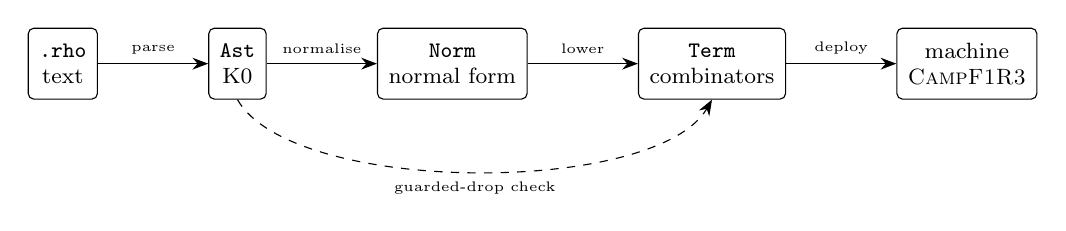
\begin{tikzpicture}[
  node distance=14mm,
  box/.style={draw, rounded corners=2pt, align=center, font=\footnotesize,
              minimum height=9mm, inner xsep=4pt},
  arr/.style={-{Stealth[length=2mm]}}]
\node[box] (txt) {\code{.rho}\\text};
\node[box, right=of txt] (ast) {\code{Ast}\\K0};
\node[box, right=of ast] (norm) {\code{Norm}\\normal form};
\node[box, right=of norm] (term) {\code{Term}\\combinators};
\node[box, right=of term] (mach) {machine\\\Camp};
\draw[arr] (txt) -- node[above, font=\tiny] {parse} (ast);
\draw[arr] (ast) -- node[above, font=\tiny] {normalise} (norm);
\draw[arr] (norm) -- node[above, font=\tiny] {lower} (term);
\draw[arr] (term) -- node[above, font=\tiny] {deploy} (mach);
\draw[arr, dashed] (ast.south) to[out=-60, in=-120, looseness=0.6]
   node[below, font=\tiny] {guarded-drop check} (term.south);
\end{tikzpicture}
\end{center}

\noindent
The dashed arc is Requirement~\ref{req:guarded}: the check reads the tree, not
the normal form, because \code{Norm::eval} has already applied
$\drp{\quo{P}} \to P$ by the time the normal form exists.

\subsection{Composing an executive}

\Fx{} gains four subcommands, alongside \code{run}, \code{show} and
\code{hash}:

\begin{center}
\begin{tabularx}{\linewidth}{@{}l>{\raggedright\arraybackslash}X@{}}
\toprule
\code{f1r3x comb} \emph{file} & Compile and print the combinator term\\
\code{f1r3x comb-hash} \emph{file} & The content hash of the compiled term\\
\code{f1r3x comb-run} \emph{file} & Compile and run; \code{--cores},
\code{--trace}, \code{--free-running} as for \code{run}\\
\code{f1r3x comb-lattice} \emph{file} & The atom multiset and the lattice
point of Section~\ref{sec:lattice}\\
\bottomrule
\end{tabularx}
\end{center}

\begin{requirement}[Core-count invariance carries over]\label{req:cores}
\code{comb-run} \MUST{} reproduce the property \code{run} already has: with
the store in its deterministic profile and a FIFO queue over encoding-ordered
components, the final scene \MUST{} be identical at one core, at sixty-four,
and free-running.
\end{requirement}

%======================================================================
\section{The lowering}\label{sec:lower}

\subsection{Phases}

\begin{enumerate}[leftmargin=1.6em]
\item \textbf{Level check} on the tree (Requirement~\ref{req:level}).
\item \textbf{Guard check} on the tree (Requirement~\ref{req:guarded}):
warnings under A, errors under B.
\item \textbf{Normalise} (\code{k1ndl1ng-norm}).
\item \textbf{Closedness check} on the normal form
(Requirement~\ref{req:closed}).
\item \textbf{Lower}, one translation unit at a time, bottom-up, memoised on
the source name (Section~\ref{sec:clauses}).
\item \textbf{Encode} and hash (Requirement~\ref{req:enc}).
\end{enumerate}

\begin{requirement}[Total and terminating]\label{req:total}
Lowering \MUST{} be total on terms that pass phases~1, 3 and~4, \MUST{}
terminate, and \MUSTNOT{} recurse on the Rust stack: the workspace's standing
rule --- an explicit stack, no recursion anywhere including \code{Drop} ---
applies here as it does to \code{k1ndl1ng-parse}.
\end{requirement}

\subsection{Occurrence analysis}\label{sec:occ}

\begin{table}[t]
\centering
\begin{tabularx}{\linewidth}{@{}llX l@{}}
\toprule
 & occurrence of $y$ & in the quoted body & link\\
\midrule
(o1) & input subject $\inp{z}{y}{S}$ & subject $\to c_{i}$ & $\bl(p_{i},c_{i})$\\
(o2) & output subject $\out{y}{S}$ & subject $\to c_{i}$ & $\br(p_{i},c_{i})$\\
(o3) & forwarded name $\out{v}{\drp{y}}$ & atom deleted & $\fw(p_{i},\enc{v})$\\
(o4) & drop $\drp{y}$ in process position & $\to \ev(c_{i})$ & $\fw(p_{i},c_{i})$\\
(o5) & inside a quotation $\quo{S}$, $y$ free in $S$ & subject $\to c_{i}$
     & constructor chain for $S$\\
\bottomrule
\end{tabularx}
\caption{The five occurrence kinds, \cite[Table~1]{draft3}.}
\label{tab:links}
\end{table}

\begin{requirement}[Classification]\label{req:classify}
For a receive with body $B$, the analysis \MUST{} walk $B$ and collect every
\code{Name::Bound(d)} whose de Bruijn index equals the number of binders
between it and the receive, and \MUST{} assign each exactly one kind by the
following disjoint test on its immediate syntactic role:
\begin{enumerate}[leftmargin=1.6em, label=(\alph*)]
\item the \code{chan} of a \code{Receive} bind, not under a quotation between
it and the receive: \textbf{o1};
\item the \code{chan} of a \code{Send}, not under a quotation: \textbf{o2};
\item the name of an \code{Eval} which is the sole argument of a \code{Send}
whose channel is not the occurrence, not under a quotation: \textbf{o3};
\item the name of an \code{Eval} in process position, not under a quotation:
\textbf{o4};
\item anywhere under a \code{Name::Quote} lying between the occurrence and the
receive: \textbf{o5}, with the chain built for the outermost such quotation.
\end{enumerate}
The tests \MUST{} be applied in this order, so that (c) takes precedence over
(d). An occurrence matching none \MUST{} raise an internal error naming the
node, never a silent default.
\end{requirement}

\begin{requirement}[Emission order]\label{req:occorder}
Occurrences \MUST{} be enumerated by ascending byte offset of their occurrence
in the encoding of the receive's body. This order is a function of the normal
form and is therefore canonical, which is what Requirement~\ref{req:paths}
needs. \cite[Def.~6.6]{draft3} says only ``let $o_{1},\dots,o_{k}$ enumerate
the free occurrences'' and leaves the order open; the order decides which
proxy is $c_{1}$, hence which seed power each link gets, hence the output
bytes.
\end{requirement}

\begin{requirement}[Coincident kinds]\label{req:coincide}
\cite[Table~1]{draft3} notes that when several kinds coincide in one atom, the
atom is deleted from the body and the links are emitted together. Each
\emph{occurrence} has exactly one kind by
Requirement~\ref{req:classify}; what coincides is several occurrences in one
atom, as in $\out{y}{\drp{y}}$. The implementation \MUST{} treat them
independently, each with its own proxy and link, in the order of
Requirement~\ref{req:occorder}, and \MUSTNOT{} fuse two occurrences into one
proxy even when the result would be smaller.
\end{requirement}

\subsection{Distributor and gate}

\begin{definition}[\cite{draft3} Def.~6.4]\label{def:gate}
For $b,c$ fresh, $G(p,S) := \sy(p,b,c) \mid \qq(b,S) \mid \ev(c)$, with $S$ a
process by Decision~\ref{dec:qsort}; and $D(x;p_{0}) := \nil$ with
$p_{0} := x$, while for $k \geq 1$
\[
  D(x;p_{0},\dots,p_{k}) := \dd(x,p_{0},q_{1}) \mid \dd(q_{1},p_{1},q_{2})
  \mid \cdots \mid \dd(q_{k-1},p_{k-1},p_{k}).
\]
\end{definition}

\begin{requirement}[Gate and distributor names]\label{req:gatenames}
$b$, $c$, the $p_{i}$ and the $q_{j}$ \MUST{} be seed powers of the unit's
seed, allocated by Requirement~\ref{req:paths}. The degenerate case $k = 0$
\MUST{} emit no duplicator and take $p_{0} := \enc{x}$ directly, as
Definition~\ref{def:gate} requires; emitting a one-way $\dd$ instead would be
correct up to $\bisim$ and would break Obligation~\ref{thm:canon} against a
compiler that did not.
\end{requirement}

\subsection{The clauses}\label{sec:clauses}

\begin{definition}[\cite{draft3} Def.~6.6, as implemented]\label{def:trans}
On names, $\enc{\quo{P}} := \quo{\enc{P}_{\quo{P}}}$
(Decision~\ref{dec:seed}). On processes,
\[
\begin{array}{rcl}
  \enc{\nil}_{s} &=& \nil\\
  \enc{P_{0} \mid \cdots \mid P_{n-1}}_{s} &=&
     \enc{P_{0}}_{s^{0}} \mid \enc{P_{1}}_{s^{10}} \mid \cdots \mid
     \enc{P_{n-1}}_{s^{1^{n-1}}}\\
  \enc{\out{x}{P}}_{s} &=& \mm(\enc{x}, \quo{\enc{P}_{s^{0}}})\\
  \enc{\inp{y}{x}{P}}_{s} &=& D(\enc{x};p_{0},\dots,p_{k}) \mid
     G(p_{0},B) \mid L_{1} \mid \cdots \mid L_{k}
\end{array}
\]
where $o_{1},\dots,o_{k}$ enumerate the free occurrences of $y$ in $P$ in the
order of Requirement~\ref{req:occorder}, each $o_{i}$ has proxy $c_{i}$,
$L_{i}$ and the residue in $B$ are given by Table~\ref{tab:links}, and $B$ is
$\enc{P}_{s^{0}}$ with every occurrence treated accordingly.
\end{definition}

\begin{requirement}[Memoisation on the name, not the position]\label{req:memo}
Lowering \MUST{} memoise translation units on the source name $\quo{P}$ ---
equivalently, on the content hash of the source normal form $P$ --- so that a
name occurring at several positions is compiled once and yields one target
name. This is Decision~\ref{dec:seed} in operational form; a position-keyed
cache instead would make the compiler non-canonical.
\end{requirement}

\subsection{Constructor chains}\label{sec:chains}

\begin{requirement}[Chain construction]\label{req:chain}
For an occurrence of kind (o5) inside the outermost enclosing quotation
$\quo{S}$, the compiler \MUST{} emit the chain rebuilding $\quo{\enc{S}}$ from
the received name and delivering it at $c_{i}$, by recursion on the path from
the occurrence to the root of $S$, per \cite[Prop.~3.9]{draft3}:
\begin{itemize}[leftmargin=1.6em]
\item at the occurrence, the value is the received name; no atom;
\item at $S' \mid S''$, emit $\cons(a,b,c)$ with the dynamic side's output at
its position and a constant message for the static side;
\item at $\out{v}{T}$, emit $\cons_{\mm}$, covering a dynamic subject, a
dynamic payload, or both;
\item at $\inp{z}{v}{T}$, emit $\cons_{\dd}$ when $z$ occurs in $T$ and
$\cons_{\sy}$ when it does not, matching the head atom of the image of the
input under Definition~\ref{def:trans};
\item every node off the path is static and is supplied as a constant message.
\end{itemize}
Chains \MUST{} be built outermost-last, so each constructor's inputs are
available before it fires.
\end{requirement}

\begin{requirement}[No repeated subject in a constructor]\label{req:norepeat}
A constructor \MUSTNOT{} be emitted with two equal argument subjects, nor with
a delivery channel equal to an input channel
(\cite[Rem.~3.4]{draft3}). Where the same value is needed twice --- as in
Example~\ref{ex:witness}, where both sides of a $\cons$ want the received
name --- the compiler \MUST{} split first with $\dd$. The store's join is over
a \emph{group} of channels; a group with a repeated channel is not a request
for two data at that channel and \MUST{} not be issued as one.
\end{requirement}

\begin{requirement}[Chain sharing]\label{req:share}
Where several (o5) occurrences lie under one quotation, the compiler \SHOULD{}
share the static constant messages and the common prefix of their chains,
splitting with $\dd$ at the deepest common node. Sharing \MUST{} be
deterministic, hence canonical, and \MUST{} be disabled by \code{--no-share}
for differential testing against the unshared form.
\end{requirement}

\subsection{Shortcuts}

\begin{requirement}[The shortcuts are feature-gated, and cost two atoms]
\label{req:shortcuts}
\cite[Rem.~6.7]{draft3} gives three cheaper special cases:
$\enc{\inp{y}{x}{\nil}} = \kk(\enc{x})$,
$\enc{\inp{y}{x}{\drp{y}}} = \ev(\enc{x})$, and
$\enc{\inp{y}{x}{\out{v}{\drp{y}}}} = \fw(\enc{x},\enc{v})$ for $v \neq y$.
They \MUST{} be behind the \code{shortcuts} feature, off by default, because
\cite[Rem.~3.10]{draft3} records that taking them puts a bound name into the
argument of an $\ev$ or a $\fw$, so the translation then needs $\cons_{\ev}$
and $\cons_{\fw}$. Enabling the feature enlarges the atom set from thirteen
shapes to fifteen, moves the lattice point, and changes every content hash. It
\MUST{} be recorded in the artefact header alongside the presentation.
\end{requirement}

\subsection{Worked examples}

\begin{example}[\cite{draft3} Ex.~6.8]\label{ex:o2}
$P = \inp{y}{a}{\out{y}{\nil}}$ has one occurrence, of kind (o2), so
\[
  \enc{P}_{s} = \dd(a,p_{0},p_{1}) \mid G(p_{0},\mm(c,\quo{\nil})) \mid
  \br(p_{1},c).
\]
Supplying $\mm(a,\quo{\enc{R}})$ gives $\mm(p_{0},\quo{\enc{R}}) \mid
\mm(p_{1},\quo{\enc{R}})$; then $\mm(c,\quo{\nil}) \mid \fw(c,\quo{\enc{R}})$;
then $\mm(\quo{\enc{R}},\quo{\nil}) = \enc{\out{\quo{R}}{\nil}}$. Note that
$\br$ yields a forwarder, per Requirement~\ref{req:departures}.
\end{example}

\begin{example}[The witness, \cite{draft3} Ex.~6.9]\label{ex:witness}
$W = \inp{y}{a}{\out{\quo{(\drp{y} \mid \drp{y})}}{\nil}}$ has one occurrence
of kind (o5), so
\[
  \enc{W}_{s} = \dd(a,p_{0},p_{1}) \mid G(p_{0},\mm(c,\quo{\nil}))
  \mid \dd(p_{1},r_{1},r_{2}) \mid \cons(r_{1},r_{2},c).
\]
The inner duplicator is Requirement~\ref{req:norepeat} in action. Receiving
$\mm(a,\quo{\enc{R}})$ builds $\mm(c,\quo{(\enc{R}\mid\enc{R})})$.
\end{example}

\begin{requirement}[Both examples are golden tests]\label{req:golden}
Examples~\ref{ex:o2} and~\ref{ex:witness} \MUST{} be checked into
\code{f1r3comb-check} as golden files: source, expected term, expected
encoding, expected content hash, and the expected reduction sequence with step
counts, for each presentation. They are the two the paper works by hand.
\end{requirement}

\subsection{Size}

\begin{requirement}[Output size]\label{req:size}
Let $k_{r}$ be the number of occurrences of the bound name in receive $r$, and
for an (o5) occurrence $o$ let $d_{o}$ be the path length from $o$ to the root
of its enclosing quotation. The compiler \MUST{} produce a term of size
\[
  |\enc{P}| \;\leq\; c\Big(|P| + \sum_{r} k_{r} + \sum_{o \in \mathrm{o5}} d_{o}\Big)
\]
and \MUSTNOT{} exhibit the quadratic name growth of \cite{rhocomb}
(\cite[Rem.~6.3]{draft3}). On the nesting family of
\cite[Prop.~8.2]{draft3} the output \MUST{} be $3d+1$ atoms against Yoshida's
$(3^{d-1}+1)/2$, tested as a law parameterised over $d$.
\end{requirement}

%======================================================================
\section{The machine}\label{sec:runtime}

\subsection{The target is store-shaped}

Every rule of Definition~\ref{def:tred} has the same form: consume a message
at each of one, two or three named subjects, and produce messages or install
atoms. There is no pattern to match beyond the subject, no binder to open, no
substitution to perform. \Camp{} is exactly a store of that shape, with joins
for the multi-subject case.

\begin{decision}[The machine is \Camp{} with a three-line matcher]
\label{dec:machine}
\code{f1r3comb-run} \MUST{} be \code{campf1r3-core::Space} instantiated over
target terms, and \MUSTNOT{} implement its own indexing, joins or replay. The
spatial matcher of \code{k1ndl1ng-campf1r3} is not used and \MUST{} not be
linked. The result is materially smaller than \Bell: no substitution, no plan
cache, no de Bruijn, no prepared continuations.
\end{decision}

\subsection{The instantiation}

\begin{center}
\begin{tabularx}{\linewidth}{@{}l>{\raggedright\arraybackslash}X@{}}
\toprule
\Camp{} parameter & \Comb{} instance\\
\midrule
$C$, channel & \code{CName}, a target name; \code{content\_hash} is
BLAKE2b-256 of its encoding (Requirement~\ref{req:neq})\\
$A$, datum & \code{enum Val \{ Loud(CName), Quiet(Term) \}} under A ---
the sorts differ, per Decision~\ref{dec:qsort}, so this is an enum over two
types and not a struct with a flag; under B, \code{Loud(Term)}\\
$P$, pattern & \code{Acc \{ accepts\_quiet: bool \}}: two values, one for
$\fw$ and one for everything else\\
$K$, continuation & \code{Rule}, the atom minus its consumed subjects\\
$M$, matcher & \code{get(p,a) = match a \{ Quiet(\_) if !p.accepts\_quiet =>
None, \_ => Some(a.clone()) \}}\\
$O$, observer & \code{NoObserver} at v1; the seam where cost accounting
attaches\\
\bottomrule
\end{tabularx}
\end{center}

\begin{requirement}[The loud/quiet distinction lives in the matcher]
\label{req:quiet}
$\qq(a,p)$ is a message only a forwarder may read
(\cite[Rem.~3.7]{draft3}). This \MUST{} be realised as the matcher rejecting a
quiet datum for a non-forwarder pattern, and \MUSTNOT{} be realised by giving
$\qq$ a different channel, which would change $\nequiv$, nor by filtering in
the machine after the store has removed the datum. The store's contract --- a
candidate that does not match is not consumed --- is what makes $\qq(b,S)$
inert in an ungated gate (\cite[Lem.~6.5]{draft3}), and that inertness is what
the release lemma rests on.
\end{requirement}

\subsection{Atoms as store operations}

\begin{center}
\begin{tabularx}{\linewidth}{@{}ll>{\raggedright\arraybackslash}X@{}}
\toprule
Atom & Store call & On commit, emit\\
\midrule
$\mm(a,v)$ & \code{produce(a, Loud(v))} & ---\\
$\qq(a,p)$ & \code{produce(a, Quiet(p))} & ---\\
$\dd(a,b,c)$ & \code{consume([a],[loud],Dup(b,c))} & $\mm(b,v) \mid \mm(c,v)$\\
$\kk(a)$ & \code{consume([a],[loud],Kill)} & $\nil$\\
$\fw(a,b)$ & \code{consume([a],[any],Fwd(b))} & $\mm(b,v)$, or
  $\mm(b,\quo{p})$ for a quiet datum\\
$\bl(a,b)$ & \code{consume([a],[loud],BindL(b))} & $\fw(v,b)$\\
$\br(a,b)$ & \code{consume([a],[loud],BindR(b))} & $\fw(b,v)$\\
$\sy(a,b,c)$ & \code{consume([a],[loud],Sync(b,c))} & $\fw(b,c)$\\
$\ev(a)$ & \code{consume([a],[loud],Eval)} & deploy the normal form of
  $\drp{v}$\\
$\cons(a,b,c)$ & \code{consume([a,b],[loud;2],ConsPar(c))} &
  $\mm(c,\quo{(p \mid r)})$\\
$\cons_{\mm}(a,b,c)$ & \code{consume([a,b],[loud;2],ConsMsg(c))} &
  $\mm(c,\quo{\mm(u,v)})$\\
$\cons_{\dd}(a,b,c,f)$ & \code{consume([a,b,c],[loud;3],ConsDup(f))} &
  $\mm(f,\quo{\dd(u,v,w)})$\\
$\cons_{\sy}(a,b,c,f)$ & \code{consume([a,b,c],[loud;3],ConsSync(f))} &
  $\mm(f,\quo{\sy(u,v,w)})$\\
\bottomrule
\end{tabularx}
\end{center}

\begin{requirement}[$\mathsf{eval}$ normalises before it deploys]
\label{req:evalnorm}
Under A the rule produces $\drp{v}$, whose normal form by
Requirement~\ref{req:dropelim} is the process $v$ quotes. The machine \MUST{}
construct $\drp{v}$ through the smart constructor, which performs the
elimination, and \MUST{} deploy the result. It \MUSTNOT{} short-circuit by
projecting the payload directly out of the name: the short-circuit is
observationally identical here and is the exact step that becomes unsound
under \code{presentation-b}, where $\drp{\quo{p}}$ and $p$ differ.
\end{requirement}

\begin{requirement}[Linear, never persistent]\label{req:linear}
Every \code{consume} \MUST{} pass \code{persist = false} and an empty
\code{PeekSet}; \code{install} \MUSTNOT{} be used. Every rule consumes both
participants, and there is no persistent atom in the calculus.
\end{requirement}

\begin{requirement}[Deploy]\label{req:deploy}
Deploying a target term \MUST{} flatten its parallel components in encoding
order --- which by Requirement~\ref{req:dropelim} is a flat multiset of atoms
with no descent case --- and issue one store call per atom, appending any
\code{CommResult} to the work queue.
\end{requirement}

\begin{requirement}[Races are scheduler choices and \MUST{} be visible]
\label{req:races}
\cite[\S3.3]{draft3} records two deliberate races: two consumers competing for
one message, and two producers competing for one consumer,
$\fw(a,b) \mid \mm(a,v) \mid \qq(a,p)$. Under the deterministic profile the
store resolves both by order key. The machine \MUST{} emit a trace event at
every such resolution, naming the alternatives not taken, so the calculus's
nondeterminism is inspectable rather than merely resolved. \Rhobots{} needs
this to draw the choice.
\end{requirement}

\subsection{Name growth}

\begin{hazard}[Names are no longer subterms of the program]\label{haz:growth}
\cite[\S12]{draft3}, open question~3: with the constructors, names grow at run
time, and $\cons$ applied to its own outputs doubles a name's size per step.
\cite[\S7]{logic} says the same thing logically: $\Cl_{S}(T)$ is an infinite
namespace with a finite presentation. Nothing the compiler emits does this,
but a received name is arbitrary and the machine must survive one.
\end{hazard}

\begin{requirement}[Interning and budget]\label{req:intern}
Constructed names \MUST{} be hash-consed: a table keyed by content hash, the
encoding stored once, channels referring to it by index. The machine \MUST{}
accept a budget --- maximum name size, maximum distinct names --- and \MUST{}
halt with \code{comb-name-budget} naming the constructor that exceeded it. The
default \SHOULD{} be generous enough that no compiled source term can reach
it, so that hitting it always means a hostile or pathological received name.
\end{requirement}

\begin{remark}
This is where the implementation repays the papers. \cite[\S12]{draft3} asks
what name growth costs in practice for the decidability of $\nequiv$ and for
cost accounting, and \cite[\S7]{logic} names it as the bridge to a graded
clause. A machine with an interning table and a counter answers it with
measurements.
\end{remark}

%======================================================================
\section{The lattice audit, and what the logic needs}\label{sec:lattice}

\cite[\S9]{draft3} organises subsets of the atom set into an expressiveness
lattice, a product of a computation axis ($\dd$, $\ev$) and a
name-construction axis ($\cons$ below $\cons_{\mm},\cons_{\dd},\cons_{\sy}$),
over a base of $\mm$ and the routers. \cite[Thm.~6.5]{logic} shows occupancy
is checkable in linear time, from the atom multiset alone. That multiset is a
fact about the compiled term, and the compiler is the only thing that knows
it.

\begin{requirement}[Reporting the point]\label{req:lattice}
\code{f1r3comb-lower} \MUST{} return, alongside the term, the multiset of atom
shapes it contains --- the $\comps{-}$ of \cite[Def.~2.9]{logic} --- and
\code{f1r3x comb-lattice} \MUST{} print the corresponding lattice point as a
pair of coordinates plus the router set. The computation \MUST{} be a count
over emitted atoms, and \MUSTNOT{} attempt to decide whether a smaller point
would suffice for the same source term, which is the open part of
\cite[\S9]{draft3}.
\end{requirement}

\begin{requirement}[The multiset is the logic's input]\label{req:logicinput}
\code{f1r3comb-term} \MUST{} expose the atom multiset and the encoding through
a stable public API, so that the occupancy checker of \cite[\S6]{logic} can be
built against it without depending on \code{f1r3comb-lower}
(Requirement~\ref{req:indep}). It \MUST{} preserve the $\mm$/$\qq$ sort
distinction in that API, since that distinction is what
\cite[Rem.~2.5]{logic} turns on, and it \SHOULDNOT{} expose anything else: the
logic's characteristic formulae, satisfaction and model checking are
\cite{logic}'s to build.
\end{requirement}

\begin{requirement}[The audit is a regression on the papers]\label{req:auditreg}
The audit \MUST{} be asserted for a corpus: a source term with no input
occupies the constructor-free point; Example~\ref{ex:o2} adds $\dd$, $\sy$,
$\ev$, $\qq$, $\br$; Example~\ref{ex:witness} adds $\cons$ and is the witness
the constructor-free fragment cannot express (\cite[Prop.~9.5]{draft3}). If a
change moves a corpus term to a different point, the change is either a bug or
a result.
\end{requirement}

\begin{remark}[A second reason for Decision~\ref{dec:presA}]
\cite[Rem.~2.7]{logic} scopes the damage carefully: occupancy, the closure
formula and the decidability results hold under either presentation, and only
three things are A-only --- the name-sort collapse, the drop-free canonical
form, and the structural visibility of the $\qq$/$\mm$ distinction. The first
two have known replacements. The third does not, and it is the one the
compiler would otherwise force on the logic.
\end{remark}

%======================================================================
\section{Correctness obligations and testing}\label{sec:test}

\begin{obligation}[Canonicity]\label{obl:canon}
Proved as Obligation~\ref{thm:canon}, and tested: for randomly generated K0
terms, and for each a random $\scong$-variant obtained by permuting parallel
components and re-associating, the compiled encodings \MUST{} be byte-equal.
\end{obligation}

\begin{obligation}[The conflation regression]\label{obl:defect}
v0.1 stated this as a test that the target congruence omits
$\drp{\quo{P}} = P$. Under Decision~\ref{dec:presA} it does not omit it, and
the test changes shape accordingly. A test \MUST{} assert that
$Q \mid \mm(\quo{Q},\quo{P})$ is stuck for a nontrivial $Q$ --- that the
machine does not implement \cite[Prop.~3.5]{draft3} --- and a second \MUST{}
assert Requirement~\ref{req:rigid}: no process is equal to an $\ev$ atom
unless it was written as one. The first is the symptom, the second the cause.
\end{obligation}

\begin{obligation}[Operational correspondence]\label{obl:opcorr}
\cite[Lem.~7.7]{draft3}: for a source communication,
$\enc{\inp{y}{x}{P}}_{s} \mid \mm(\enc{x},\quo{\enc{R}}) \wred T$ with
$T \bisim \enc{P\{\quo{R}/y\}}_{s}$ in $k+3$ steps followed by at most $k$
administrative steps. The machine \MUST{} be tested against both halves: step
counts exactly, for a corpus with known $k$; and the residue by differential
testing. Note that \cite[Lem.~7.7]{draft3}'s (o4) case now holds under either
presentation --- under A both sides deliver $\drp{\quo{\enc{R}}}$, which the
equation makes equal to $\enc{R}$.
\end{obligation}

\begin{obligation}[Differential testing against \Bell]\label{obl:diff}
For a corpus of K0 programs, run the source under \Bell{} and the compiled
term under \code{f1r3comb-run}, both deterministic, to quiescence, and compare
observations. The observation \MUST{} be the multiset of messages at names
that are encodings of source names --- the encoded observer class of
\cite[Thm.~7.9]{draft3} --- and \MUSTNOT{} include the seed-derived apparatus,
which by \cite[Lem.~7.6]{draft3} no encoded context can name. A mismatch
\MUST{} report the first divergent step of both traces.
\end{obligation}

\begin{obligation}[A against B]\label{obl:AB}
The corpus \MUST{} be run under both presentations and the observations
compared. \cite[Def.~3.3]{draft3} asserts that no rule, lemma or proof
distinguishes them; this is that assertion made executable, and it is the
check that the \code{presentation-b} seam has not rotted. The encodings will
differ and \MUST{} be expected to; only the observations are compared.
\end{obligation}

\begin{obligation}[Golden encodings]\label{obl:goldenenc}
Every example in this specification and in \cite[\S6]{draft3} \MUST{} be a
golden file with source, term, encoding and hash, per presentation, and the
goldens \MUST{} be regenerated only by an explicit command.
\end{obligation}

\begin{obligation}[Property tests]\label{obl:prop}
A generator for K0 terms \MUST{} exist, and on its output: lowering is total;
the term contains no target variable (Requirement~\ref{req:novars}) and, under
A, no drop (Requirement~\ref{req:dropelim}); no constructor has a repeated
subject or a delivery channel among its inputs
(Requirement~\ref{req:norepeat}); every seed power is outside the constructor
image (Requirement~\ref{req:seedimage}); the size bound of
Requirement~\ref{req:size} holds; deploy-then-quiesce terminates for
terminating sources.
\end{obligation}

\begin{obligation}[Seed independence, as a property]\label{obl:seedind}
\cite[Lem.~7.8]{draft3} says two seeds give bisimilar terms. The compiler
never uses two seeds for one name, but the property is worth testing as a
check on the machine: compile with the term-determined seed and with an
injected alternative, run both, compare observations. A failure here is a
machine bug, not a compiler bug.
\end{obligation}

%======================================================================
\section{Errors and diagnostics}\label{sec:errors}

\begin{requirement}[Diagnostic model]\label{req:diag}
Diagnostics \MUST{} follow \cite[\S9]{k1ndl1ng}: a stable code, a span, a
message, no panic on any input, and every independent error reported in one
pass.
\end{requirement}

\begin{center}
\begin{tabularx}{\linewidth}{@{}ll>{\raggedright\arraybackslash}X@{}}
\toprule
Code & Phase & Meaning\\
\midrule
\code{comb-level} & 1 & A form above K0; names the level that would accept it\\
\code{comb-unguarded-drop} & 2 & A drop of a name not bound by an enclosing
input; warning under A, error under B\\
\code{comb-drop-quote} & 2 & A literal $\drp{\quo{Q}}$; collapsed by the
equation under A, unsound under B\\
\code{comb-open} & 4 & A free variable or free name survived grounding\\
\code{comb-unforgeable} & 4 & An unforgeable name; no target former\\
\code{comb-occ-unclassified} & 5 & Internal: an occurrence matching no kind\\
\code{comb-presentation-mismatch} & deploy & Artefact compiled under the other
presentation (Requirement~\ref{req:pseam})\\
\code{comb-feature-mismatch} & deploy & Artefact compiled with a different
\code{shortcuts} setting\\
\code{comb-name-budget} & run & Name size or count budget exceeded\\
\code{comb-decode} & any & A source tag, or the drop tag in an A build, where
a target tag was expected (Requirements~\ref{req:tags},
\ref{req:droptag})\\
\bottomrule
\end{tabularx}
\end{center}

%======================================================================
\section{Performance, portability, dependencies}\label{sec:perf}

\begin{requirement}[Complexity]\label{req:complexity}
Lowering \MUST{} be $O(n \log n)$ in the size of the normal form, the $\log$
from the memo table of Requirement~\ref{req:memo}, plus the chain term of
Requirement~\ref{req:size}. Encoding \MUST{} be linear and computed once per
node. A machine step \MUST{} be $O(1)$ expected in the size of the store. The
atom multiset of Requirement~\ref{req:lattice} \MUST{} be linear, matching
\cite[Thm.~6.5]{logic}.
\end{requirement}

\begin{requirement}[Targets]\label{req:targets}
On the reference machine of \cite[\S11]{k1ndl1ng}: compile a $10^{4}$-node
source term in under 10\,ms; deploy $10^{5}$ atoms in under 100\,ms; sustain
$10^{6}$ machine steps per second free-running. Budget figures for a first
implementation, to be re-stated once measured.
\end{requirement}

\begin{requirement}[Portability]\label{req:port}
Every crate \MUST{} build for \code{wasm32-unknown-unknown} without
\code{wasm-bindgen}, \MUST{} carry \code{forbid(unsafe\_code)}, and \MUSTNOT{}
take an external dependency. Hashing comes from \code{k1ndl1ng-norm}.
\end{requirement}

\begin{requirement}[Determinism]\label{req:det}
Given the same source, presentation and configuration, the compiled term, its
encoding, its hash, the event stream and the final scene \MUST{} be
bit-identical across runs, hosts, core counts and WebAssembly versus native.
\end{requirement}

%======================================================================
\section{What the implementation asks of the papers}\label{sec:paper}

Two items from v0.1 are discharged by draft~3's revision and are recorded as
closed: the binder rules now produce forwarders and the arity slips in $\fw$
and in the constructors' delivery channel are fixed
(\cite[Rem.~3.4]{draft3}); and the presentation question, which v0.1 met only
obliquely, is now posed explicitly. The rest stand.

\begin{enumerate}[leftmargin=1.8em]

\item \textbf{The implementation argument for B does not hold}
(Section~\ref{sec:s4rebuttal}). \cite[\S4]{draft3} reads the F1R3FLY
normaliser as evidence for B. Sorting a parallel composition is the monoid
laws, common to both presentations; de Bruijn indexing applies to source
binders and the combinators have none; and the one presentation-specific
rewrite the code performs, $\drp{\quo{P}} \to P$, is A's equation. Proposed
amendment: keep \S4's structural argument, which is sound, and withdraw the
appeal to the implementation, or restate it as what a future optimising
decoder would need.

\item \textbf{Seed powers are constructible} (Erratum~\ref{err:seed}).
$s^{w0} = \quo{\mm(s^{w},\quo{\nil})}$ is in the image of $\cons_{\mm}$.
Proposed amendment: $s^{w0} = \quo{\bl(s^{w},s^{w})}$. \cite[Lem.~6.2]{draft3}
is unchanged; the freshness it gives becomes freshness against reachable
names, which is the property the constructors make relevant.

\item \textbf{The seed of a quotation must be term-determined}
(Decision~\ref{dec:seed}). \cite[Def.~6.6]{draft3}'s ``$w$ is the position of
that quotation in the enclosing term'' makes one source name compile to
several target names. Proposed amendment:
$\enc{\quo{P}} := \quo{\enc{P}_{\quo{P}}}$, which
\cite[Lem.~6.2]{draft3} already licenses.

\item \textbf{The enumeration order of occurrences is observable}
(Requirement~\ref{req:occorder}). Proposed amendment: fix it, or state that
the translation is defined only up to the induced bijection on proxies.

\item \textbf{Coincident occurrence kinds} (Requirement~\ref{req:coincide}).
\cite[Table~1]{draft3}'s note is about occurrences, not kinds. Proposed
amendment: say so, and say whether fusing two occurrences into one proxy is
permitted.

\item \textbf{The shortcuts change the atom set}
(Requirement~\ref{req:shortcuts}). \cite[Rem.~3.10]{draft3} says it;
\cite[Rem.~6.7]{draft3} offers the shortcuts without repeating it. Proposed
amendment: cross-reference them.

\item \textbf{The formation table's $\mm$ row is presentation-specific.}
\cite[Rem.~2.6]{logic} already raises this and this specification seconds it
from the implementation side: \cite[\S3.2]{draft3} presents formation as
common to both presentations while sorting the message payload as a name,
which is A's sorting, and \S3.3 then re-sorts it. Proposed amendment: split
the row, as \cite[Def.~2.3]{logic} does.

\item \textbf{The source calculus of \cite[\S2]{draft3} is not the source
calculus of \cite[Def.~2.6]{k1ndl1ng}} (Obligation~\ref{obl:srcagree}). The
first omits $\drp{\quo{P}} \scong P$ and uses semantic substitution; the
second asserts it and \code{Norm::eval} applies it. They agree on
guarded-drop terms, which is why the mismatch has gone unremarked. Proposed
amendment: state the agreement as a lemma in \S2, since with
Decision~\ref{dec:presA} the target now satisfies the equation and the source
presentation is the last place it does not.

\end{enumerate}

%======================================================================
\section{Open questions and deferred work}

\begin{enumerate}[leftmargin=1.8em]
\item \textbf{Name growth, measured} (Hazard~\ref{haz:growth}). The machine is
the instrument \cite[\S12]{draft3} question~3 and \cite[\S7]{logic} both want.
\item \textbf{The quiet constructors} (\cite[Rem.~7.12]{draft3}). Should every
constructor have a quiet variant emitting $\qq(c,\cdot)$? Under
Decision~\ref{dec:qsort} the loud and quiet cases are already two arms of one
enum, so a \code{quiet-constructors} feature is cheap to try, and
Obligation~\ref{obl:diff} says whether an encoded observer can tell.
\item \textbf{Receptivity.} \cite[open item~5]{logic}. If the logic gains
$\rcp{\phi}\psi$, the $\mm$/$\qq$ argument for A weakens and the presentation
question is worth reopening. Until then it is the decisive argument.
\item \textbf{An optimising decoder.} Remark~\ref{rem:whatAcosts}: the one
development that would force B. If a backend that discharges administrative
forwarders at decode time is wanted, it is a \code{presentation-b} backend,
and Obligation~\ref{obl:AB} is what keeps that path open.
\item \textbf{The constructors-only presentation}
(\cite[\S10]{draft3}). Deferred until observation is defined over the
constructor family.
\item \textbf{Composition with the $\pi$ compiler.} \cite{nowns} encodes $\pi$
into rho; composing gives $\pi$ into the combinators. The composite's
canonicity is a new obligation, not an inherited one.
\item \textbf{A decompiler.} A term in the image of $\enc{-}$ should be
recoverable, and a round-trip test would be a strong canonicity check;
whether the image is decidable is open.
\end{enumerate}

%======================================================================
\section{Delivery}

\begin{center}
\begin{tabularx}{\linewidth}{@{}ll>{\raggedright\arraybackslash}X@{}}
\toprule
M & Deliverable & Done when\\
\midrule
M0 & \code{f1r3comb-term} & Sorts, atom enum, drop elimination, encoding,
hash, printer, decoder, atom multiset; tag-disjointness and rigidity tests;
round-trip property test\\
M1 & \code{f1r3comb-lower}, no (o5) & Level, guard and closedness checks;
seeds; kinds (o1)--(o4); Example~\ref{ex:o2} golden; canonicity property test\\
M2 & Constructor chains & Kind (o5),
Requirements~\ref{req:chain}--\ref{req:share}; Example~\ref{ex:witness}
golden; lattice audit and the public API of
Requirement~\ref{req:logicinput}\\
M3 & \code{f1r3comb-space}, \code{f1r3comb-run} & Matcher, rule table, deploy,
scheduler, trace; conflation regression; step-count tests\\
M4 & \code{f1r3comb-check} & Differential testing against \Bell; the A/B
comparison; corpus; size and complexity tests\\
M5 & \Fx{} subcommands, WASM & \code{comb}, \code{comb-hash}, \code{comb-run},
\code{comb-lattice}; \code{wasm32} build; performance measured and
Requirement~\ref{req:targets} re-stated\\
\bottomrule
\end{tabularx}
\end{center}

\noindent
M0 through M2 are the compiler and are independently useful: they give
\cite{logic} a term type and an atom multiset, and they give draft~3 a
machine-checked version of its own examples. The \code{presentation-b} seam is
built at M0 and exercised at M4; it is not a separate milestone, and it will
rot if Obligation~\ref{obl:AB} is not run.

%======================================================================
\section{Changes from v0.1}\label{sec:v1delta}

\begin{center}
\begin{tabularx}{\linewidth}{@{}l>{\raggedright\arraybackslash}X@{}}
\toprule
v0.1 & v0.2\\
\midrule
No presentation question & Section~\ref{sec:which}: A chosen, B behind
\code{presentation-b}, with the \cite[\S4]{draft3} argument answered\\
Hazard: \code{Norm::eval} applies a fatal equation & Not a hazard under A;
one rewrite, sound on both sides. The hazard returns under B
(Requirement~\ref{req:nodropB})\\
Requirement: target congruence omits $\drp{\quo{P}} = P$ &
Requirement~\ref{req:noconflation}: the drop and the guard are distinct
constructors. The equation is optional; the conflation is the defect\\
Guarded-drop check is a gating phase & A diagnostic under A, gating under B
(Requirement~\ref{req:guarded}), with
Obligation~\ref{obl:srcagree} explaining why\\
Decision: $\qq$ carries a name & Withdrawn. $\qq$ carries a process and the
sort asymmetry is load-bearing (Decision~\ref{dec:qsort},
Remark~\ref{rem:reverse})\\
Datum: name plus a \code{quiet} flag & A two-case enum over two sorts\\
Tag table: no drop, $\cons_{\mid}$ & Drop tag reserved and rejected under A;
$\cons$ per \cite[\S3.2]{draft3}; $\ev$ given its own tag distinct from the
drop\\
Lattice audit only & Plus Requirement~\ref{req:logicinput}: the multiset and
the sort distinction are a public API for \cite{logic}\\
Six items asked of the paper & Eight, of which two from v0.1 are discharged
by draft~3's revision and three are new\\
Cross-references to draft~3 & Renumbered throughout against the revision;
\cite{logic} added\\
\bottomrule
\end{tabularx}
\end{center}

%======================================================================
\begin{thebibliography}{99}

\bibitem{BIHOL} C.\,B. Wells, M. Stay and L.\,G. Meredith.
\emph{Behavior in higher-order languages: admissible observers, relative
pushouts, and the encoding of extended theories.} In preparation,
F1R3FLY.io, 2026.

\bibitem{bytecode} F1R3FLY.io.
\emph{Bytecode or normal form: what the executive should execute.}
\code{publications/campf1r3/bytecode-or-normal-form}, 2026.

\bibitem{campf1r3} F1R3FLY.io.
\emph{CampF1R3: an in-memory tuple space.}
\code{publications/campf1r3/campf1r3-spec}, 2026.

\bibitem{draft3} L.\,G. Meredith and M. Stay.
\emph{Name-free combinators for the rho calculus: a repair, a linear encoding,
and the one operation that was missing.} Draft~3,
\code{publications/rho-combinators}, September 2026.

\bibitem{logic} F1R3FLY.io.
\emph{A spatial-behavioural logic for the rho combinators: structural
formulae, one context modality, and decidable occupancy of the expressiveness
lattice.} Draft~2, \code{publications/rho-combinators}, September 2026.

\bibitem{k1ndl1ng} F1R3FLY.io.
\emph{K1ndl1ng: a parser and a normaliser for the kernel of rholang served by
CampF1R3, as composable crates.} Specification v0.2,
\code{publications/campf1r3/k1ndl1ng-spec}, 17 September 2026.

\bibitem{MeredithRadestock05} L.\,G. Meredith and M. Radestock.
\emph{A reflective higher-order calculus.} ENTCS 141(5):49--67, 2005.

\bibitem{nowns} L.\,G. Meredith.
\emph{Namespaces without a name server: freshness by communication, and a
fully abstract encoding of the $\pi$-calculus in the rho calculus.}
\code{publications/pi2rhobugfix}, F1R3FLY.io, 2026.

\bibitem{rhocomb} L.\,G. Meredith and M. Stay.
\emph{Name-free combinators for concurrency.} Working draft, \code{rho4u}.

\bibitem{Yoshida02} N. Yoshida.
\emph{Minimality and separation results on asynchronous mobile processes:
representability theorems by concurrent combinators.}
Theoretical Computer Science 274(1--2):231--276, 2002.

\end{thebibliography}

\end{document}
